%%%%%%%%%%%%%%%%%%%%%%%%%%%%%%%%%%%%%%%%%%%%%%%%%%%%%%%%%% 
\chapter{組合せ遷移問題} \label{chap:background}
%%%%%%%%%%%%%%%%%%%%%%%%%%%%%%%%%%%%%%%%%%%%%%%%%%%%%%%%%% 

\section{組合せ遷移問題}
組合せ遷移問題(\cite{Ito18:tohoku})は基となる探索問題が存在し,探索問題の実行可能解,及び\textbf{隣接関係}により定義される.
組合せ遷移問題を定義することは,基となる探索問題が形成する\textbf{解空間グラフ}を定義することに等しい.
ここで,解空間グラフの頂点は,基となる探索問題の実行可能解である. 
また,解空間グラフの辺は,隣接関係が成立つ2つの実行可能解に対応する頂点の間に存在する.
本論文では,このようにして定義される解空間グラフ上の2つの頂点間の到達可能性についてを対象とする.

組合せ遷移問題の基となる探索問題には,充足可能性判定問題(SAT),独立集合問題,グラフ点彩色問題などが存在する.
このような組合せ遷移問題の中には\textbf{PSPACE完全}であるものも存在する. 
PSPACEは問題の難易度を表すクラスの1つであり,属する問題は指数時間で解けることが知られている. 
現在,P $\subseteq$ NP $\subseteq$ PSPACEであることが知られている.

実社会において,組合せ遷移問題は持続可能なシステムへの応用されている. 
解空間グラフ上において2つの頂点に経路があるならば,探索問題における制限をみたしたままある状態から別の状態へと遷移可能である. 
これは,システムの正常性を維持したまま異なる状態へと変化可能であることを意味する.

\section{$k$彩色遷移問題}
$k$彩色遷移問題(\cite{BC2009:tcs})とは組合せ遷移問題の一種であり,\textbf{グラフ点彩色問題}を基としている. 
グラフ点彩色問題はグラフ$G=(V, E)$と色数$k$が与えられたとき,辺が存在する頂点同士が異なる色になるように各頂点に1つの色を割当てることが可能かの判定問題である. 
例として,図~\ref{fig:ex_graph}のグラフを$k=3$で彩色したときの実行可能解の一例を図~\ref{fig:graph_col}に示す. 
ここで,頂点の枠外に書かれた$v_i$は各頂点の番号を表す.
また,頂点の枠内に書かれた$c_i$はそれぞれの頂点が色$i$で塗られることを表す.

\begin{figure}[htbp]
  \centering
  \begin{tabular}{c}
    
    \begin{minipage}{0.45\hsize}
      \centering
      %%%%%%%%%%%%%%%%%%%%%%%%%%%%%%%%%%%%%%%%%%%%%%%%%%
% 実行例(t=0) (第6章で使う)
%%%%%%%%%%%%%%%%%%%%%%%%%%%%%%%%%%%%%%%%%%%%%%%%%%

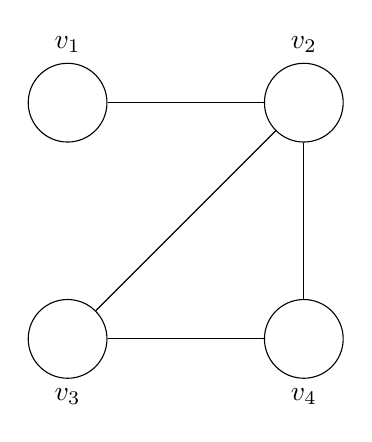
\begin{tikzpicture}[x=1.5cm, y=1.5cm]

  % 設定
  \tikzset{node/.style={circle,draw=black,minimum size=1cm}}
 

 
  % 補助線
  % \draw [help lines,blue] (0,0) grid (20,6);
 
  % node %
  \node[node, label=above:$v_1$] at (-1,1) (node1) {};
  \node[node, label=above:$v_2$] at (1,1) (node2) {};
  \node[node, label=below:$v_3$] at (-1,-1) (node3) {};
  \node[node, label=below:$v_4$] at (1,-1) (node4) {};
 
  \foreach \u / \v in {node1/node2, node2/node3, node2/node4, node3/node4}
  \draw (\u) -- (\v);
 \end{tikzpicture}
 
 %%%%%%%%%%%%%%%%%%%%%%%%%%%%%%%%%%%%%%%%%%%%%%%%%%%%%%%%%%
 %%% Local Variables:
 %%% mode: japanese-latex
 %%% TeX-master: paper.tex
 %%% End:
 
      \caption{グラフ}
      \label{fig:ex_graph}
    \end{minipage}

    \begin{minipage}{0.45\hsize}
      \centering
      %%%%%%%%%%%%%%%%%%%%%%%%%%%%%%%%%%%%%%%%%%%%%%%%%%
% 実行例(t=0) (第6章で使う)
%%%%%%%%%%%%%%%%%%%%%%%%%%%%%%%%%%%%%%%%%%%%%%%%%%

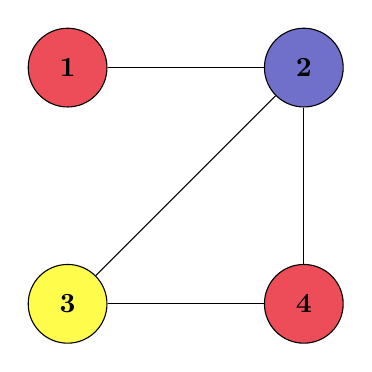
\begin{tikzpicture}[x=1.5cm, y=1.5cm]

  % 設定
  \tikzset{node/.style={circle,draw=black,minimum size=1cm}}
 
  % 色
  \definecolor{red}{RGB}{230,0,18}
  \definecolor{blue}{RGB}{51,51,179}
  \definecolor{yellow}{RGB}{255,251,0}
 
  % 補助線
  % \draw [help lines,blue] (0,0) grid (20,6);
 
  % node %
  \node[node, fill=red!70] at (-1,1) (node1) {\textbf{1}};
  \node[node, fill=blue!70] at (1,1) (node2) {\textbf{2}};
  \node[node, fill=yellow!70] at (-1,-1) (node3) {\textbf{3}};
  \node[node, fill=red!70] at (1,-1) (node4) {\textbf{4}};
 
  \foreach \u / \v in {node1/node2, node2/node3, node2/node4, node3/node4}
  \draw (\u) -- (\v);
 \end{tikzpicture}
 
 %%%%%%%%%%%%%%%%%%%%%%%%%%%%%%%%%%%%%%%%%%%%%%%%%%%%%%%%%%
 %%% Local Variables:
 %%% mode: japanese-latex
 %%% TeX-master: paper.tex
 %%% End:
 
      \caption{$k=3$における彩色例}
      \label{fig:graph_col}
    \end{minipage}

  \end{tabular}  
\end{figure}

$k$彩色遷移問題ではグラフ$G$と色数$k$に加え,$G$の$k$色彩色の2つの実行可能解$\alpha$(初期状態),$\beta$(目標状態)が与えられる. 
このとき,その他の実行可能解は与えられない. 
解空間グラフの頂点は,$G$の$k$彩色における実行可能解となる.
また,隣接関係はある1つの頂点のみにおいて色が異なる実行可能解の間で成立ち,解空間グラフの辺は隣接関係が成立つ場合にのみ存在する.
以上の条件において,$G$の$k$色彩色問題から形成される解空間グラフ上で初期状態に対応する頂点から目標状態に対応する頂点への到達可能性が問われる. 
例として,グラフを図~\ref{fig:ex_graph},$k=4$,初期状態を図~\ref{fig:recol_s},目標状態を図~\ref{fig:recol_g}としたものを示す.

\begin{figure}[htbp]
  \centering
  \begin{tabular}{c}

    \begin{minipage}{0.45\hsize}
      \centering
      %%%%%%%%%%%%%%%%%%%%%%%%%%%%%%%%%%%%%%%%%%%%%%%%%%
% 実行例(t=0) (第6章で使う)
%%%%%%%%%%%%%%%%%%%%%%%%%%%%%%%%%%%%%%%%%%%%%%%%%%

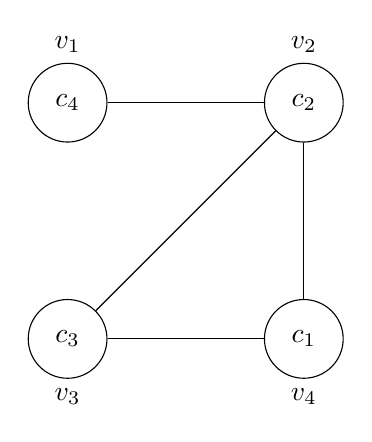
\begin{tikzpicture}[x=1.5cm, y=1.5cm]

  % 設定
  \tikzset{node/.style={circle,draw=black,minimum size=1cm}}
 

 
  % 補助線
  % \draw [help lines,blue] (0,0) grid (20,6);
 
  % node %
  \node[node, label=above:$v_1$] at (-1,1) (node1) {$c_4$};
  \node[node, label=above:$v_2$] at (1,1) (node2) {$c_2$};
  \node[node, label=below:$v_3$] at (-1,-1) (node3) {$c_3$};
  \node[node, label=below:$v_4$] at (1,-1) (node4) {$c_1$};
 
  \foreach \u / \v in {node1/node2, node2/node3, node2/node4, node3/node4}
  \draw (\u) -- (\v);
 \end{tikzpicture}
 
 %%%%%%%%%%%%%%%%%%%%%%%%%%%%%%%%%%%%%%%%%%%%%%%%%%%%%%%%%%
 %%% Local Variables:
 %%% mode: japanese-latex
 %%% TeX-master: paper.tex
 %%% End:
 
      \caption{初期状態}
      \label{fig:recol_s}
    \end{minipage}

    \begin{minipage}{0.45\hsize}
      \centering
      %%%%%%%%%%%%%%%%%%%%%%%%%%%%%%%%%%%%%%%%%%%%%%%%%%
% 実行例(t=0) (第6章で使う)
%%%%%%%%%%%%%%%%%%%%%%%%%%%%%%%%%%%%%%%%%%%%%%%%%%

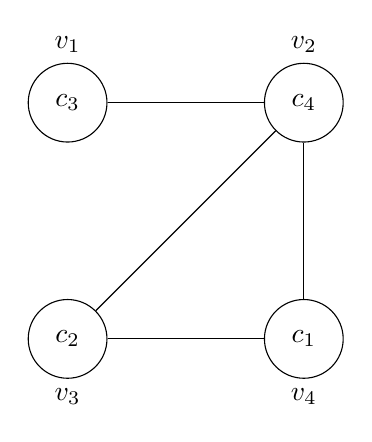
\begin{tikzpicture}[x=1.5cm, y=1.5cm]

  % 設定
  \tikzset{node/.style={circle,draw=black,minimum size=1cm}}
 

 
  % 補助線
  % \draw [help lines,blue] (0,0) grid (20,6);
 
  % node %
  \node[node, label=above:$v_1$] at (-1,1) (node1) {$c_3$};
  \node[node, label=above:$v_2$] at (1,1) (node2) {$c_4$};
  \node[node, label=below:$v_3$] at (-1,-1) (node3) {$c_2$};
  \node[node, label=below:$v_4$] at (1,-1) (node4) {$c_1$};
 
  \foreach \u / \v in {node1/node2, node2/node3, node2/node4, node3/node4}
  \draw (\u) -- (\v);
 \end{tikzpicture}
 
 %%%%%%%%%%%%%%%%%%%%%%%%%%%%%%%%%%%%%%%%%%%%%%%%%%%%%%%%%%
 %%% Local Variables:
 %%% mode: japanese-latex
 %%% TeX-master: paper.tex
 %%% End:
 
      \caption{目標状態}
      \label{fig:recol_g}
    \end{minipage}
    
  \end{tabular}
\end{figure}

\noindent
解となる遷移系列を図~\ref{fig:ans_varrecol}に示す. $t=0$と$t=1$では,頂点$v_1$の色のみが変化していることがわかる. 
同様に,$t=1$から$t=2$,$t=2$から$t=3$においても1つの頂点のみ色が変化してる. 
また各$t$において,グラフ点彩色の定義を満たしていることがわかる.

\begin{figure}[htbp]
  \centering
  \begin{subfigure}{0.4\hsize}
    \centering
    %%%%%%%%%%%%%%%%%%%%%%%%%%%%%%%%%%%%%%%%%%%%%%%%%%
% 実行例(t=0) (第6章で使う)
%%%%%%%%%%%%%%%%%%%%%%%%%%%%%%%%%%%%%%%%%%%%%%%%%%

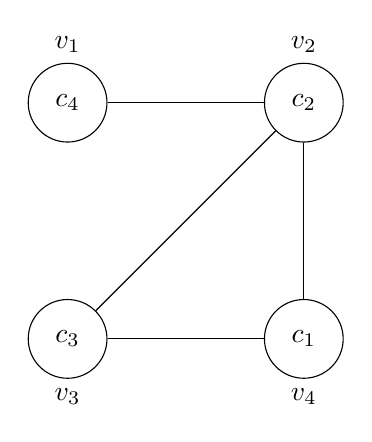
\begin{tikzpicture}[x=1.5cm, y=1.5cm]

  % 設定
  \tikzset{node/.style={circle,draw=black,minimum size=1cm}}
 

 
  % 補助線
  % \draw [help lines,blue] (0,0) grid (20,6);
 
  % node %
  \node[node, label=above:$v_1$] at (-1,1) (node1) {$c_4$};
  \node[node, label=above:$v_2$] at (1,1) (node2) {$c_2$};
  \node[node, label=below:$v_3$] at (-1,-1) (node3) {$c_3$};
  \node[node, label=below:$v_4$] at (1,-1) (node4) {$c_1$};
 
  \foreach \u / \v in {node1/node2, node2/node3, node2/node4, node3/node4}
  \draw (\u) -- (\v);
 \end{tikzpicture}
 
 %%%%%%%%%%%%%%%%%%%%%%%%%%%%%%%%%%%%%%%%%%%%%%%%%%%%%%%%%%
 %%% Local Variables:
 %%% mode: japanese-latex
 %%% TeX-master: paper.tex
 %%% End:
 
    \caption{$t=0$ (初期状態)}
   \end{subfigure}
   \hspace{1cm}
   \begin{subfigure}{0.4\hsize}
    \centering
    %%%%%%%%%%%%%%%%%%%%%%%%%%%%%%%%%%%%%%%%%%%%%%%%%%
% 実行例(t=0) (第6章で使う)
%%%%%%%%%%%%%%%%%%%%%%%%%%%%%%%%%%%%%%%%%%%%%%%%%%

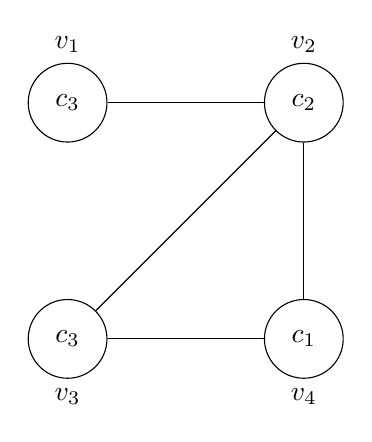
\begin{tikzpicture}[x=1.5cm, y=1.5cm]

  % 設定
  \tikzset{node/.style={circle,draw=black,minimum size=1cm}}
 

 
  % 補助線
  % \draw [help lines,blue] (0,0) grid (20,6);
 
  % node %
  \node[node, label=above:$v_1$] at (-1,1) (node1) {$c_3$};
  \node[node, label=above:$v_2$] at (1,1) (node2) {$c_2$};
  \node[node, label=below:$v_3$] at (-1,-1) (node3) {$c_3$};
  \node[node, label=below:$v_4$] at (1,-1) (node4) {$c_1$};
 
  \foreach \u / \v in {node1/node2, node2/node3, node2/node4, node3/node4}
  \draw (\u) -- (\v);
 \end{tikzpicture}
 
 %%%%%%%%%%%%%%%%%%%%%%%%%%%%%%%%%%%%%%%%%%%%%%%%%%%%%%%%%%
 %%% Local Variables:
 %%% mode: japanese-latex
 %%% TeX-master: paper.tex
 %%% End:
 
    \caption{$t=1$}
   \end{subfigure}
   \\
   \begin{subfigure}{0.4\hsize}
    \centering
    %%%%%%%%%%%%%%%%%%%%%%%%%%%%%%%%%%%%%%%%%%%%%%%%%%
% 実行例(t=0) (第6章で使う)
%%%%%%%%%%%%%%%%%%%%%%%%%%%%%%%%%%%%%%%%%%%%%%%%%%

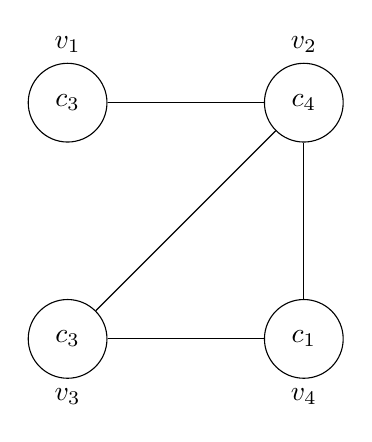
\begin{tikzpicture}[x=1.5cm, y=1.5cm]

  % 設定
  \tikzset{node/.style={circle,draw=black,minimum size=1cm}}
 

 
  % 補助線
  % \draw [help lines,blue] (0,0) grid (20,6);
 
  % node %
  \node[node, label=above:$v_1$] at (-1,1) (node1) {$c_3$};
  \node[node, label=above:$v_2$] at (1,1) (node2) {$c_4$};
  \node[node, label=below:$v_3$] at (-1,-1) (node3) {$c_3$};
  \node[node, label=below:$v_4$] at (1,-1) (node4) {$c_1$};
 
  \foreach \u / \v in {node1/node2, node2/node3, node2/node4, node3/node4}
  \draw (\u) -- (\v);
 \end{tikzpicture}
 
 %%%%%%%%%%%%%%%%%%%%%%%%%%%%%%%%%%%%%%%%%%%%%%%%%%%%%%%%%%
 %%% Local Variables:
 %%% mode: japanese-latex
 %%% TeX-master: paper.tex
 %%% End:
 
    \caption{$t=2$}
   \end{subfigure}
   \hspace{1cm}
   \begin{subfigure}{0.4\hsize}
    \centering
    %%%%%%%%%%%%%%%%%%%%%%%%%%%%%%%%%%%%%%%%%%%%%%%%%%
% 実行例(t=0) (第6章で使う)
%%%%%%%%%%%%%%%%%%%%%%%%%%%%%%%%%%%%%%%%%%%%%%%%%%

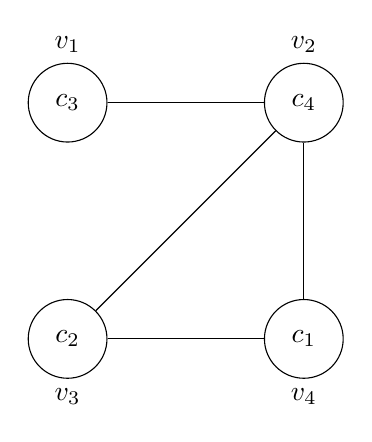
\begin{tikzpicture}[x=1.5cm, y=1.5cm]

  % 設定
  \tikzset{node/.style={circle,draw=black,minimum size=1cm}}
 

 
  % 補助線
  % \draw [help lines,blue] (0,0) grid (20,6);
 
  % node %
  \node[node, label=above:$v_1$] at (-1,1) (node1) {$c_3$};
  \node[node, label=above:$v_2$] at (1,1) (node2) {$c_4$};
  \node[node, label=below:$v_3$] at (-1,-1) (node3) {$c_2$};
  \node[node, label=below:$v_4$] at (1,-1) (node4) {$c_1$};
 
  \foreach \u / \v in {node1/node2, node2/node3, node2/node4, node3/node4}
  \draw (\u) -- (\v);
 \end{tikzpicture}
 
 %%%%%%%%%%%%%%%%%%%%%%%%%%%%%%%%%%%%%%%%%%%%%%%%%%%%%%%%%%
 %%% Local Variables:
 %%% mode: japanese-latex
 %%% TeX-master: paper.tex
 %%% End:
 
    \caption{$t=3$ (目標状態)}
   \end{subfigure}

   \caption{遷移系列の例}
   \label{fig:ans_varrecol}
\end{figure}

$k$彩色遷移問題の難しさは,色数$k$によって変化することが知られている. 
\begin{itemize}
  \item $k = 2$のとき,グラフは2部グラフであり明らかに到達可能ではない.
  \item $k = 3$のとき,多項式時間で判定可能である. \cite{CHM2008:iwoca}
  \item $k \geq 4$のとき,PSPACE完全である. \cite{BC2009:tcs}
\end{itemize}
また,グラフと色数に制限を加えた場合,多項式時間で解けるものが存在する. \cite{BC2009:tcs}
\begin{itemize}
  \item グラフが平面グラフであり$k \geq 7$のとき,多項式時間で解くことが可能である.
  \item グラフが平面2部グラフであり$k \geq 5$のとき,多項式時間で解くことが可能である.
\end{itemize}
しかし,汎用的かつ効率的なアルゴリズムはいまだ発見されていない.

%%% Local Variables:
%%% mode: latex
%%% TeX-master: "paper"
%%% End:
